\section{Reguleringsteknikk}
\subsection{Blokkskjema for et reguleringssystem}
$$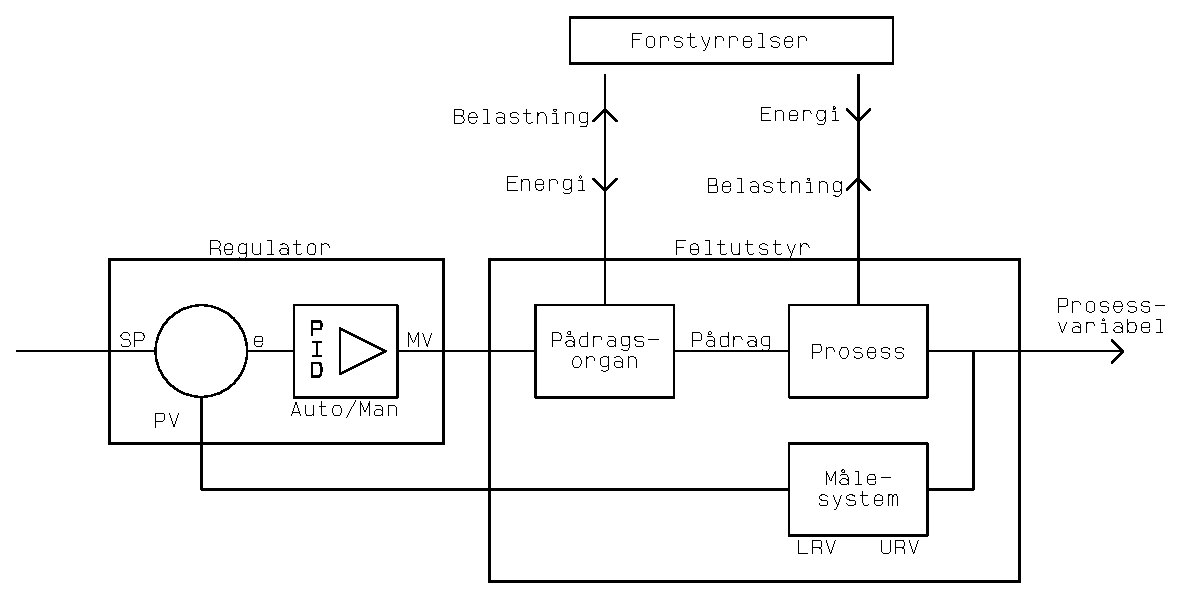
\includegraphics[width=1\textwidth]{./regblock.eps}$$

\vskip 5pt 
Direktevirkende regulator og reverstert regulator

\vskip 5pt 
En reversvirkende regulator er satt opp slik at pådraget øker når
PV er mindre enn SP. $e=SP-PV$

\vskip 5pt 
En direktevirkende regulator er satt opp slik at pådraget øker når
PV er større enn SP. $e=PV-SP$
\vfil \eject
\subsection{Optimalisering}
\subsubsection{Tims rule of tumb}
\begin{enumerate}
	\item Bare jobb med en justering av et parameter om gangen. Når du justerer flere mister du kontrollen. 
	\item Proporsjonalleddet bestemmer hvor fort en prosess går mot settpunktet. Stor proporsjonalforsterkning vil få prosesse til å nå settpunktet raskt, men du vil få et oversving og mest sannsynlig oscillasjoner. Om du setter P-forsterkningen for lavt unngår du oscillasjoner men det vil ta lang tid å nå settpunktet. Start med I-leddet og D-leddet avslått og øk forsterkningen forsiktig  fra 0.25 (0.25, 0.5, 1, 2, 4, 8, 16) til du får oscillasjoner. Reduser så forsterkningen litt. En regulator med bare P-ledd vil ha et statisk avvik fra settpunktet. 
	\item I-leddet virker ved å fjerne feil. Det kan hjelpe til med å redusere oscillasjoner og statiske avvik, men feil justering vil føre til oversving og oscillasjoner. Reduser I-tiden i forsiktig til oscillasjoner og statisk avvik er elliminert. 
	\item D-leddet er ikke nødvendig i de fleste tilfeller om det er akseptabelt med oversving. Om du trenger D-leddet øk forsiktid d-tiden til du er fornød med responsen på variasjoner i prosessen  (SP forandringer).
\end{enumerate}





\subsubsection{Ziegler\_nichols svingemetode}
\begin{enumerate}
\item Regulatoren må stå i manuell modus.
\item Få prosessen til arbidpunktet ved å justere MV manuelt eller ved å bruke en ikke optimalisert regulering. Det er viktig at PV er tilnærmet lik SP da prosessen kan ha andre egenskaper ved andre verdier. 
\item Sett regulatoren til å bare bruke P-leddet. Sett I-ledd til uendelig eller så høyt den går. NB noen regulatorer slår av I-leddet om du setter I-tiden til 0, sjekk  manualen. Sett D-leddet til 0. 
\item Sett regulatoren i automatisk modus.
\item Øk $K_p$ (du kan starte med $K_p$ = 1) inntil det oppstår stående svingninger
i sløyfen etter et sprang i settpunktet. (Reguleringssystemet er da
på stabilitetsgrensen.) Spranget skal være lite, f.eks. 5\% av referansens
verdiområde, slik at prosessen holder seg nokså nær arbeidspunktet.
Men spranget må heller ikke være så lite at responsen ikke kan observeres.
Obs: Pass på at pådraget ikke når sine metningsgrenser (maks, min)
under eksperimentene. Hvis pådraget når en av disse grensene,
vil det kunne bli stående svingninger uansett hvor stor K p vi bruker.
F.eks. kan vi da ha funnet at K pk = 1000000 gir stående svingninger,
og ihht. formelen for K p i en PI-regulator skal da K p settes lik
450000, som temmelig sikkert gir et ustabilt reguleringssystem! Det
gjelder altså å finne den minste K p u som gir stående svingninger
uten at pådraget når metningsgrensene. Dette krever at du overvåker
pådraget under eksperimentene og passer på å ikke ha så store settpunktsendringer
at pådraget når maksimum- eller minimumsverdiene.
\item Noter $K_p$ -verdien som gir stående svingninger. Denne verdien kalles
	den kritiske forsterkning $K_{Pu}$. Noter også perioden $P_u$ for de stående
svingningene. Denne perioden kalles den kritiske perioden.
\item Beregn regulatorparametrene i henhold til tabellen  og legg dem
inn i regulatoren. Forhåpentligvis får da reguleringssystemet tilfredsstillende
ytelse. Er stabiliteten i reguleringssløyfen dårlig (store oversving
i responsene), er det enklest å prøve å redusere $K_p$ .
\end{enumerate}
\begin{tabular}{|c|c|c|c|}
\hline 
 &  &  & \tabularnewline
\hline 
P-regulator & 0.5$K_{pk}$ & $\infty$ & 0\tabularnewline
\hline 
PI-regulator & 0.45$K_{pk}$ & $\frac{P_{u}}{1.2}$ & 0\tabularnewline
\hline 
PID-regulator & 0.6$K_{pk}$ & $\frac{P_{u}}{2}$ & $\frac{P_{u}}{8}=\frac{T_{i}}{4}$\tabularnewline
\hline 
\end{tabular}




\subsubsection{Skogestads metode}

Skogestad har angitt PID-regulatorinnstilling for en rekke ulike prosesstyper. Vi bruker den på følgende prosesstyper:
\begin{itemize}
\item Selvstabiliserende med tidsforsinkelse. (Eksempel på
prosess med slik dynamikk er varmeveksler.)
\item Selvstabiliserende med neglisjerbar tidsforsinkelse. Ved denne type prossess vil Z\&N være vanskelig å få til å svinge
\item Integrerende med tidsforsinkelse 
(Eksempel: Tank med transportbånd, som flistanken.)
\item Integrerende uten tidsforsinkelse (Eksempel: Væsketank styrt av pumpe eller ventil på inn- eller utløp.)
\end{itemize}

\paragraph{Innstilling av PI-regulator for tidkonstant med tidsforsinkelse}

~

\includegraphics{Sprang_selvregulerende.eps}

\[
K_{P}=\dfrac{\tau}{K\left(T_{C}+\theta\right)}
\]

\[
T_{i}=min[\tau,c(T_{c}+\theta]
\]

Her bruker en den minste verdien av $\tau$ og c (c er 2 eller 4)

\includegraphics[width=1\textwidth]{Reg_step_response01}

Her er et eksempel på en prosess med tidsforsinkelse. Når vi leser
av garfen får vi at

\begin{eqnarray*}
\theta & = & 0.5s\\
\tau & = & 5s\\
K & = & 2
\end{eqnarray*}

Det gir oss:
\[
K_{P}=\dfrac{\tau}{K\left(T_{C}+\theta\right)}=\dfrac{5}{2(0.5+0.4)}=2.5
\]

c=2 er her mindre en T=5 som gir 
\[
T_{i}=c(T_{c}+\theta)=2(0.5+0.5)=2
\]

Det gir følgende innregulering på et sprang fra 50 til 55. 

\includegraphics[width=1\textwidth]{Reg_innreg_skogestad01}

\paragraph{Innstilling av PI-regulator for integrator med tidsforsinkelse}

~

\includegraphics{Sprang_integrerendeprosess.eps}

\[
K_{i}=\dfrac{\Delta PV}{\Delta MV\cdot\Delta t}
\]

\[
Kp=\dfrac{1}{K_{i}\left(T_{c}+\theta\right)}
\]

\[
T_{i}=c\left(T_{c}+\theta\right)
\]

Eksempel:

\includegraphics[width=1\textwidth]{Reg_step_integrator}

\[
K_{i}=\dfrac{\Delta PV}{\Delta MV\cdot\Delta t}=\dfrac{40\%}{5\%\cdot8s}=1/s
\]
\[
\tau=0.5s
\]

\[
Kp=\dfrac{1}{K_{i}\left(T_{c}+\theta\right)}=\dfrac{1}{1}
\]

\[
T_{i}=c\left(T_{c}+\theta\right)=2\left(0.5+0.5\right)=2
\]
Som gir følgende innregulering

\includegraphics[width=1\textwidth]{Reg_innreg_skogestad02}
\vfil  \eject
